\subsection{Chain of Responsability}
\label{chain-of-responsability}

\textbf{Scopo}: Comportamentale \\
\textbf{Raggio d'azione}: Oggetti

\paragraph{Definizione} Il pattern Chain of Responsability permette di evitare l'accoppiamento di una richiesta del mittente e del destinatario, facendo in modo che entrambi riescano ad averla esaudita. Consente di passare le richieste lungo una catena di gestori. Dopo aver ricevuto una richiesta, ciascun gestore decide di elaborarla o di trasmetterla al gestore successivo nella catena.

\paragraph{Motivazione} Consideriamo un sistema di aiuto contestuale per un'interfaccia grafica utente in cui l'utente può ottenere informazioni di aiuto su qualsiasi parte dell'interfaccia semplicemente cliccandoci sopra. L'aiuto fornito dipende dalla parte dell'interfaccia selezionata e dal suo contesto; per esempio, un pulsante in una finestra di dialogo potrebbe avere informazioni di aiuto diverse da un pulsante simile nella finestra principale. Se non esistono informazioni di aiuto specifiche per quella parte dell'interfaccia, il sistema dovrebbe mostrare un messaggio di aiuto più generale sul contesto immediato, come l'intera finestra di dialogo. È quindi naturale organizzare le informazioni di aiuto secondo la loro generalità, dalla più specifica alla più generale. Inoltre, è chiaro che una richiesta di aiuto viene gestita da uno tra diversi oggetti dell'interfaccia utente, e quale oggetto dipende dal contesto e da quanto specifica sia l'informazione di aiuto disponibile. Il problema qui è che l'oggetto che alla fine fornisce l'aiuto non è conosciuto esplicitamente dall'oggetto (ad esempio il pulsante) che inizia la richiesta di aiuto.

\begin{multicols}{2}
    \begin{figure}[H]
        \centering
        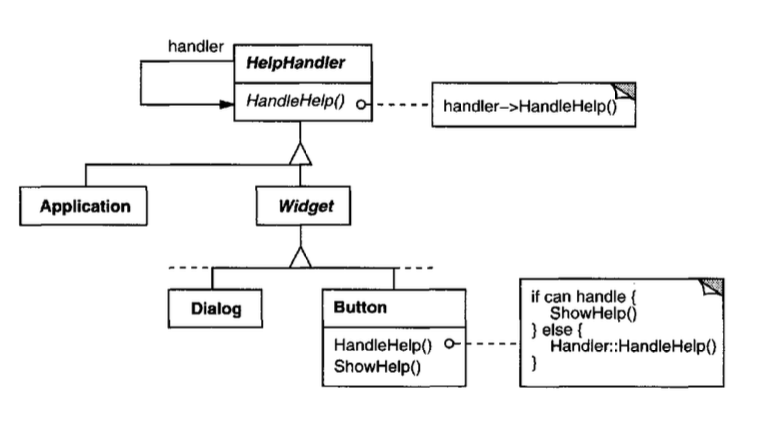
\includegraphics[width=1\linewidth]{assets/pattern/chain-of-responsability/cor-esempio-class.png}
    \end{figure}
    \columnbreak
    \begin{figure}[H]
        \centering
        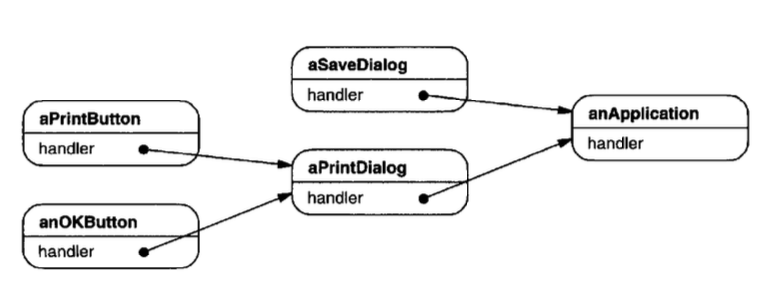
\includegraphics[width=1\linewidth]{assets/pattern/chain-of-responsability/cor-esempio-object.png}
    \end{figure}
\end{multicols}

Quello di cui abbiamo bisogno è un modo per disaccoppiare il pulsante che inizia la richiesta dagli oggetti che potrebbero fornire le informazioni di aiuto. Il pattern Chain of Responsibility definisce come questo accada. L'idea di questo pattern è disaccoppiare mittenti e destinatari dando a più oggetti la possibilità di gestire una richiesta. La richiesta viene passata lungo una catena di oggetti finché uno di essi non la gestisce. Il primo oggetto nella catena riceve la richiesta e o la gestisce o la inoltra al prossimo candidato nella catena, che fa altrettanto. L'oggetto che ha fatto la richiesta non ha conoscenza esplicita di chi la gestirà—diciamo che la richiesta ha un destinatario implicito.

\paragraph{Applicabilità} È consigliabile utilizzare il pattern Chain of Responsability quando:
\begin{itemize}
    \item Più di un oggetto può gestire una richiesta e il gestore non è noto a priori, ma dovrebbe essere determinato automaticamente;
    \item Si vuole inviare una richiesta a uno dei diversi oggetti senza specificare esplicitamente il destinatario;
    \item L'insieme di oggetti in grado di gestire una richiesta dovrebbe essere specificato dinamicamente;
\end{itemize}

\begin{figure}[H]
    \centering
    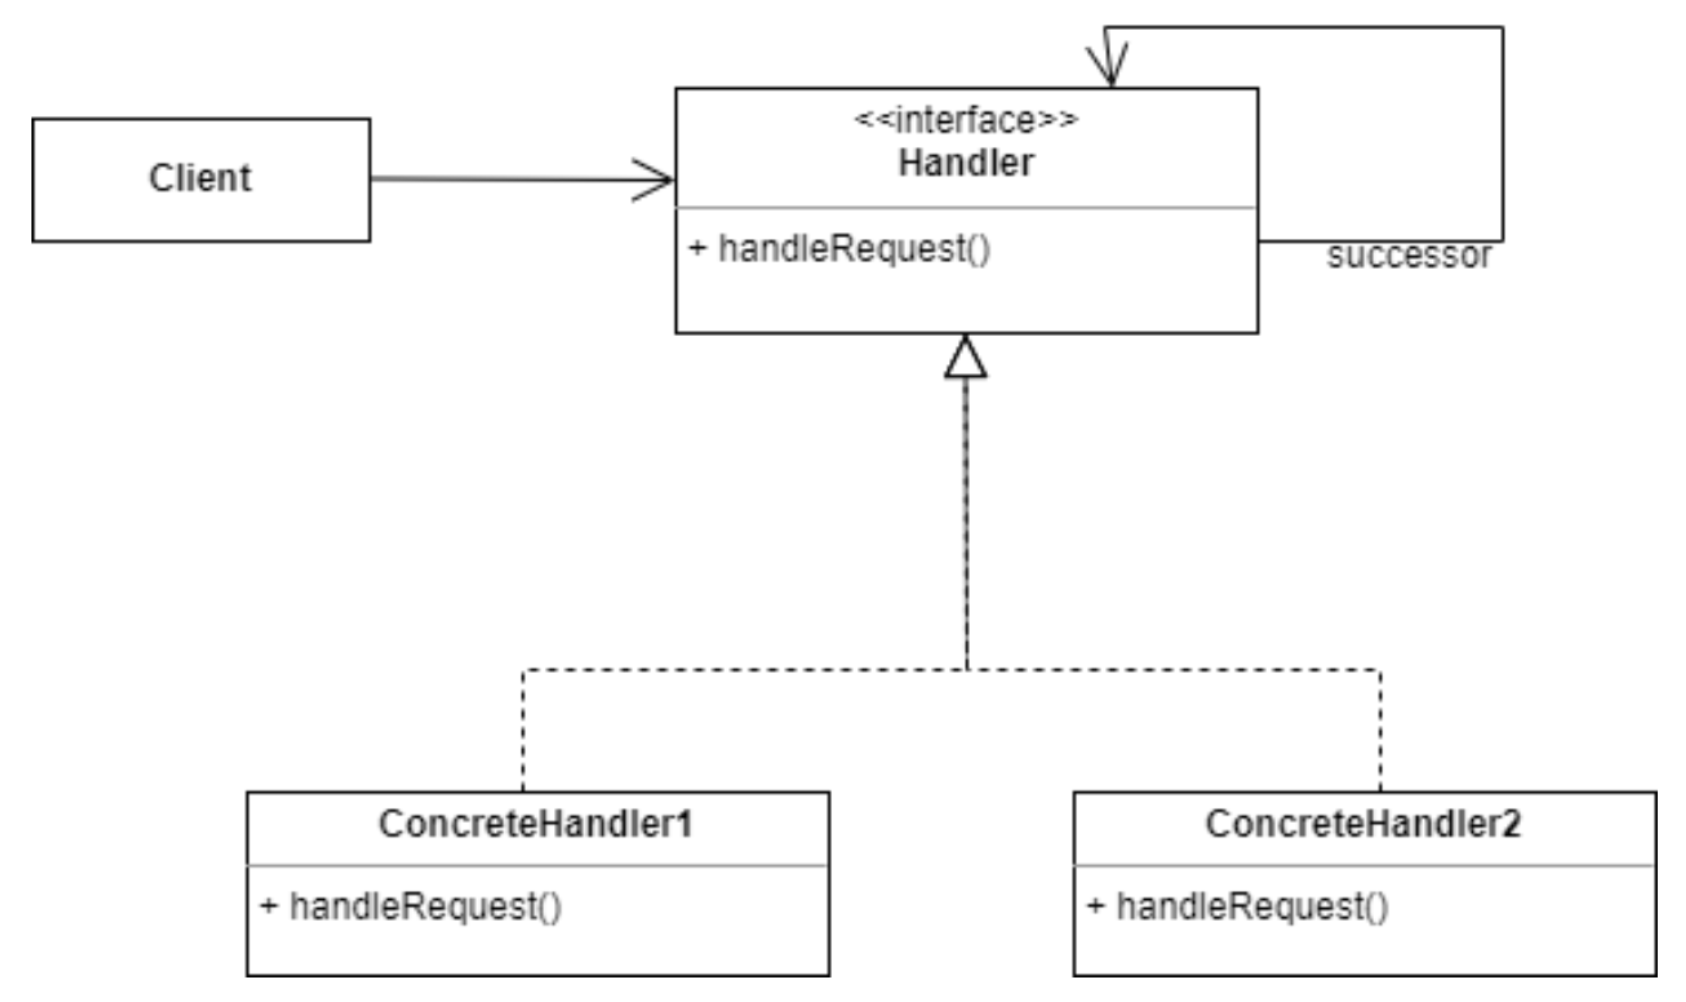
\includegraphics[width=0.5\linewidth]{assets/pattern/chain-of-responsability/cor-struttura.png}
    \caption{Class Diagram del pattern CoR}
\end{figure}

\paragraph{Struttura} I partecipanti del pattern sono:
\begin{itemize}
    \item  \textbf{Handler} (HelpHandler): definisce un'interfaccia per la gestione delle richieste e può indicare il collegamento successivo;
    \item \textbf{ConcreteHandler} (PrintButton, PrintDialog): gestisce le richieste di cui è responsabile, può accedere al suo successore, se è in grado di gestire la richiesta lo fa, altrimenti inoltra la richiesta al suo successore;
    \item \textbf{Client}: avvia la richiesta a un oggetto ConcreteHandler sulla catena;
\end{itemize}

Quando un Client invia una richiesta, questa viene propagata lungo la catena fino a quando un oggetto ConcreteHandler non si assume la responsabilità di gestirla.

\begin{figure}[H]
    \centering
    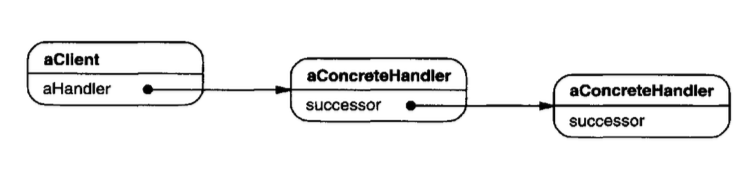
\includegraphics[width=0.5\linewidth]{assets/pattern/chain-of-responsability/cor-object-diagram.png}
\end{figure}

\paragraph{Conseguenze} Il pattern Chain of Responsability consente quindi di:
\begin{itemize}
    \item Ridurre l'accoppiamento;
    \item Avere maggiore flessibilità nell'assegnazione delle responsabilità agli oggetti;
\end{itemize}

È bene sapere che la ricezione di una richiesta non è garantita poiché una richiesta non ha un destinatario esplicito.

\begin{figure}[H]
    \centering
    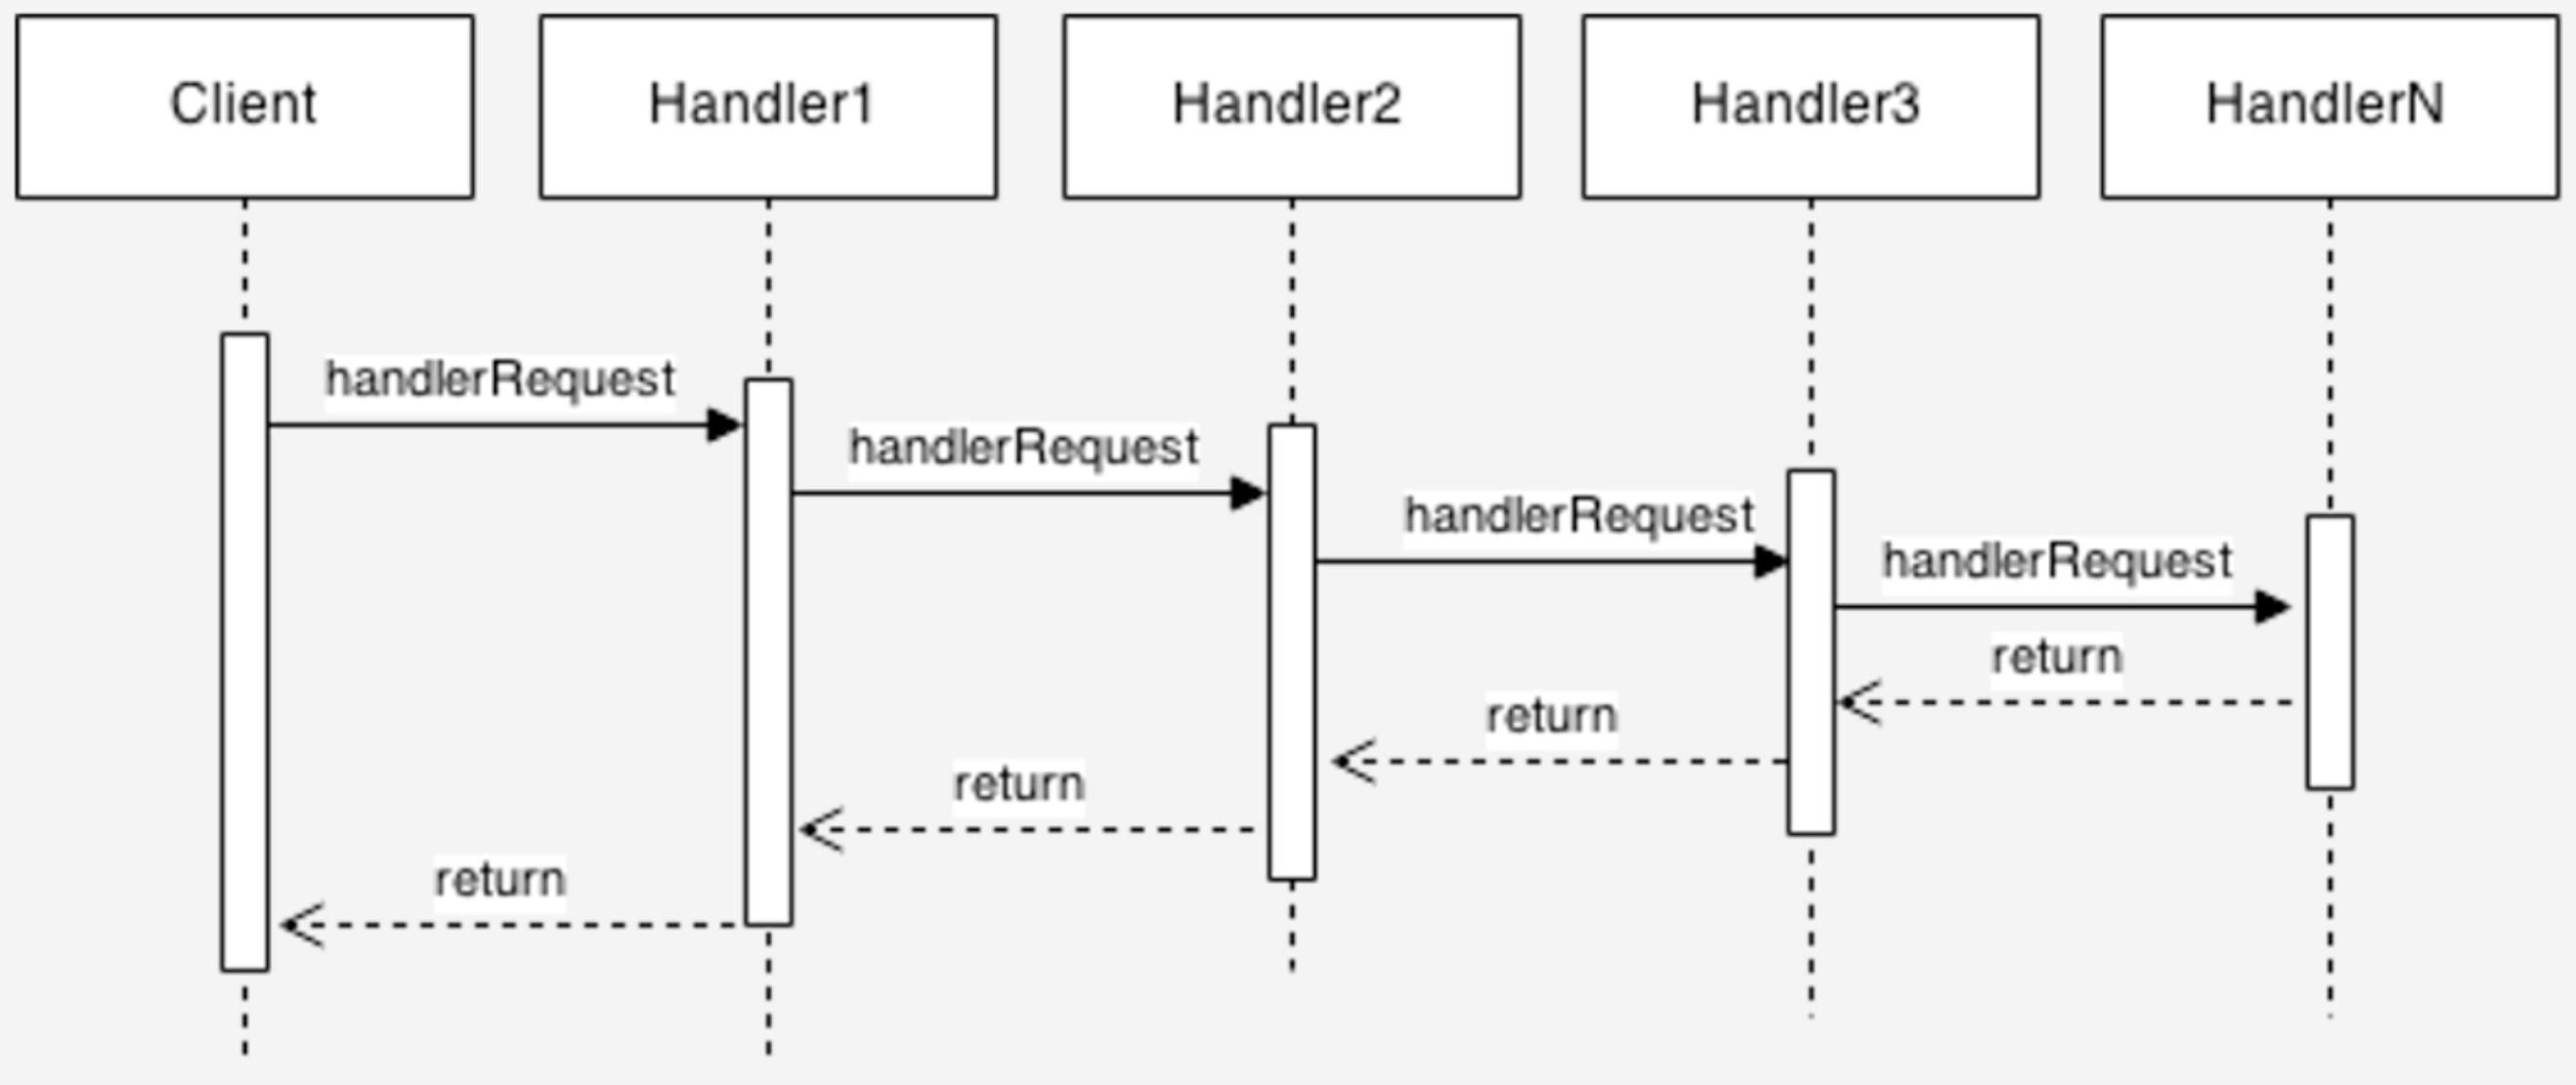
\includegraphics[width=0.75\linewidth]{assets/pattern/chain-of-responsability/cor-sequence.png}
    \caption{Sequence Diagram del patter CoR}
\end{figure}

\newpage